% https://tex.stackexchange.com/questions/51757/how-can-i-use-tikz-to-make-standalone-svg-graphics
\documentclass{standalone}
\usepackage[svgnames]{xcolor} % Enabling colors by their 'svgnames'
\usepackage{tikz}
\usetikzlibrary{calc}
\usepackage{amsmath,amsfonts,amsthm}
\usepackage{physics}

\begin{document}
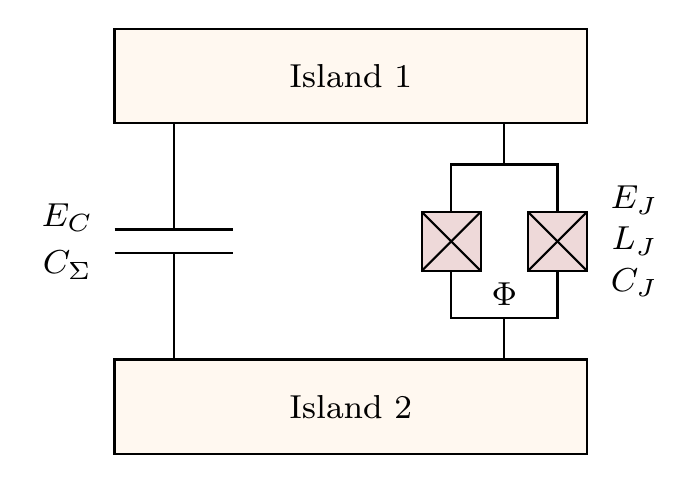
\begin{tikzpicture}[scale=1.5, every node/.style={scale=1.5}]
    %Capacitor
    \draw[thick] (0,0.1) -- (1,0.1);
    \draw[thick] (0,-0.1) -- (1,-0.1);
    
    % Left top cable
    \draw[thick] (0.5,0.1) -- (0.5,1);
    % Left bottom cable
    \draw[thick] (0.5,-0.1) -- (0.5,-1);
    
    %Top island
    \filldraw[thick, fill=DarkOrange!6] (0,1) rectangle (4,1.8);
    %Bottom island
    \filldraw[thick, fill=DarkOrange!6] (0,-1) rectangle (4,-1.8);
    
    %Double Josephson junction.
    
    \draw[thick] (3.3,1) -- (3.3, 0.65); %Top stick
    \draw[thick] (3.3,-1) -- (3.3, -0.65); %Lower stick
    
    \draw[thick] (2.85,0.25) -- (2.85,0.65) -- (3.75,0.65) -- (3.75,0.25);
    \draw[thick] (2.85,-0.25) -- (2.85,-0.65) -- (3.75,-0.65) -- (3.75,-0.25);
    
    %Right box
    \filldraw[thick, fill=DarkRed!15] (3.5,-0.25) rectangle (4,0.25); 
    \draw[thick] (3.5,0.25) -- (4,-0.25); %Top-low diagonal
    \draw[thick] (3.5,-0.25) -- (4,0.25); %Low-top diagonal
    
    %Left box
    \filldraw[thick, fill=DarkRed!15] (2.6,-0.25) rectangle (3.1,0.25); 
    \draw[thick] (2.6,0.25) -- (3.1,-0.25); %Top-low diagonal
    \draw[thick] (2.6,-0.25) -- (3.1,0.25); %Low-top diagonal
    
    
    %Text
    \node at (2, 1.4) {\footnotesize Island 1};
    \node at (2,-1.4) {\footnotesize Island 2};
    
    \node at (-0.4,0.2) {\footnotesize $E_C$};
    \node at (-0.4,-0.2) {\footnotesize $C_\Sigma$};
    
    \node at (4.4,0.35) {\footnotesize $E_J$};
    \node at (4.4,0) {\footnotesize $L_J$};
    \node at (4.4,-0.35) {\footnotesize $C_J$};
    
    \node at (3.3,-0.45) {\footnotesize $\Phi$};
    
\end{tikzpicture}
\end{document}


